%%%%%%%%%%%%%%%%%%%%%%%%%%%%%%%%%%%%%%%%%%%%%%%%%%%%%%%%%%%%%%%%%%%%%%%%%%%%%%%
% SECTION 2: The Problem & Representation Learning
%%%%%%%%%%%%%%%%%%%%%%%%%%%%%%%%%%%%%%%%%%%%%%%%%%%%%%%%%%%%%%%%%%%%%%%%%%%%%%%
\section{The Problem}

% The Dominant Paradigm
\begin{frame}{The Dominant Paradigm Before Deep Learning}
    \textbf{Hand-engineered features:}
    \begin{itemize}
        \item A human expert decides what the machine should measure
        \item A \textbf{linear classifier} computes weighted sum against threshold
    \end{itemize}
    
    \vspace{1em}
    \textbf{Example: HOG (Histogram of Oriented Gradients)}
    \begin{enumerate}
        \item Compute edge directions at each pixel
        \item Build histograms per cell
        \item Feed resulting vector to SVM
    \end{enumerate}
    
    \vspace{1em}
    \textit{Every new problem needed new hand-crafted features}
\end{frame}

% SVM Decision Boundary - Classic vs Deep Learning
\begin{frame}{Linear vs Learned Decision Boundaries}
    \begin{center}
        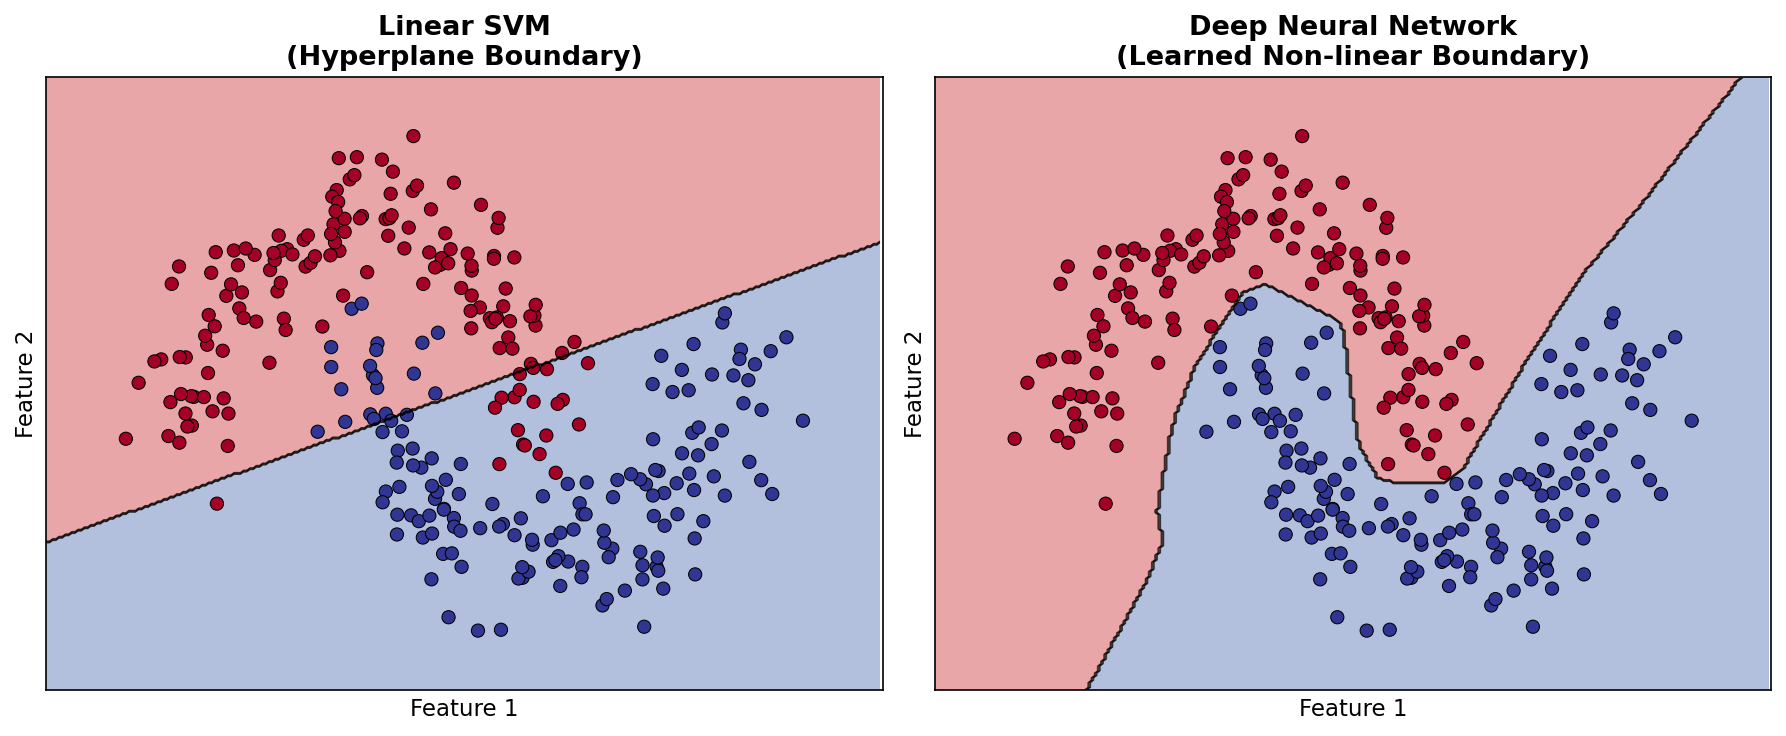
\includegraphics[width=0.95\textwidth]{figures/svm_vs_deep.png}
    \end{center}
    
    \vspace{0.5em}
    Deep learning learns \textbf{non-linear transformations}, making complex boundaries possible
\end{frame}

% The Fundamental Limit
\begin{frame}{The Fundamental Limit}
    \textbf{Known since the 1960s:}
    \begin{itemize}
        \item Linear classifiers can only partition space into \textbf{half-spaces separated by a hyperplane}
        \item Complex, curved, or nested decision boundaries are impossible
        \item No matter the scale, there are functions a linear classifier cannot learn
    \end{itemize}
    
    \vspace{1em}
    \textbf{The question:}
    
    \textit{What if the machine learned the features itself?}
\end{frame}

% What is Deep Learning?
\begin{frame}{What is Deep Learning?}
    \textbf{Deep learning}: representation learning with \textbf{multiple levels of abstraction}
    
    \vspace{1em}
    \begin{itemize}
        \item Neural networks with many layers (``deep'')
        \item Each layer transforms the representation
        \item Higher layers = more abstract features
    \end{itemize}
    
    \vspace{1em}
    \textbf{Key insight:}
    \begin{quote}
        ``Deep learning methods are representation-learning methods with multiple levels of representation, obtained by composing simple but non-linear modules.''
    \end{quote}
\end{frame}

% Representation Learning
\begin{frame}{Representation Learning}
    \begin{quote}
        ``Representation learning is a set of methods that allows a machine to be fed with raw data and to automatically discover the representations needed for detection or classification.''
    \end{quote}
    
    \vspace{1em}
    \begin{itemize}
        \item Rather than hand-crafting features, \textbf{train the system to discover them}
        \item Each layer learns increasingly abstract representations:
    \end{itemize}
    
    \begin{center}
        \texttt{Raw pixels → Edges → Shapes → Parts → Objects}
    \end{center}
\end{frame}

% Why Depth Matters
\begin{frame}{Why Depth Matters}
    \textbf{Two compounding advantages:}
    
    \vspace{1em}
    \textbf{1. Combinatorial capacity}
    \begin{itemize}
        \item With $n$ binary features: $2^n$ possible configurations
        \item 30 neurons can distinguish over 1 billion concepts
    \end{itemize}
    
    \vspace{1em}
    \textbf{2. Exponential expressiveness}
    \begin{itemize}
        \item Each additional layer \textbf{multiplies} expressive power
        \item A shallow network needs exponentially more neurons to match a deep one
    \end{itemize}
    
    \vspace{1em}
    \textbf{Depth is a qualitative difference, not merely quantitative}
\end{frame}
